\documentclass{article}
\usepackage[utf8]{inputenc}
\usepackage{graphicx}
\usepackage{parskip}
\usepackage{textcomp}
\usepackage{hyperref}
\hypersetup{
    colorlinks=true,
    linkcolor=blue,
    filecolor=magenta,      
    urlcolor=cyan,
}
\usepackage{listings}
\lstset{language=C,
                basicstyle=\ttfamily,
                keywordstyle=\color{blue}\ttfamily,
                stringstyle=\color{red}\ttfamily,
                commentstyle=\color{green}\ttfamily,
                morecomment=[l][\color{magenta}]{\#}
}

\title{The Vending Machine Controller - RTOS}
\author{By \\ Umang Deshpande and Akshay Hegde}
\date{June 2017}

\begin{document}
\maketitle

\section{Objectives}
\begin{itemize}
    \item Understanding the RTOS implementation
    \item Implementing a Vending Machine Model
\end{itemize}
\section{Prerequisites}
\begin{itemize}
    \item Basics of RTOS, familiarization with tasks, semaphores and task scheduling.
    \item Drawing up of a statechart from the problem statement. (Please go through Resources in the Resources section for the same)
    \item Understanding of Statemachine implementation of switch debouncing.
\end{itemize}
\section{Problem Statement}
\qquad The overall objective is to design a vending machine controller. 
\begin{enumerate}
\item The system has five digital inputs and three digital outputs. You can simulate the system with five switches and three LEDs.
\item The inputs are quarter , dime , nickel , soda and diet . The quarter input will go high, then go low when a 25¢ coin is added to the machine. The dime and nickel inputs work in a similar manner for the 10¢  and 5¢ coins.
\item The sodas cost 35¢ each. The user presses the soda button to select a regular soda and the diet button to select a diet soda.
\item The GiveSoda output will release a regular soda if pulsed high, then low. Similarly, the GiveDiet output will release a diet soda if pulsed high, then low. The Change output will release a 5¢ coin if pulsed high, then low.
\end{enumerate}
So from user perspective, user inserts desired amount of coins and select Diet or Regular soda for taking out soda from vending machine.

\section{Relevant Theory}
\subsection{Statechart Implementation}
\qquad Vending Machine has 4 states of operation. \textit{INITM, COIN, SELECT} and \textit{DELIVERY}.
\subsubsection{INITM:}
\begin{itemize}
    \item Initially controller will be in INITM state.
    \item Perform reset/initialization of requisite variables(coins entered, number of soda cans selected, etc.).
    \item Transition immediately to the next state, i.e.,\textit{COIN}.
\end{itemize}

\subsubsection{COIN:}
\begin{itemize}
    \item Instructions for coin entry and mapped switch presses should be displayed on screen.(As in Fig 1)
    \item Depending upon which switch is pressed, increment the total sum. Ex:
    for \textit{DIME} coin entered, \textit{sum} = \textit{sum} + 5.
    \item Display total money entered till now. (As in Fig 2, Fig 3 and Fig 4)
    \item Switch press is used to transition to next mode. Remain in \textit{COIN} mode till mode transition switch is pressed.
\end{itemize}
\begin{center}
   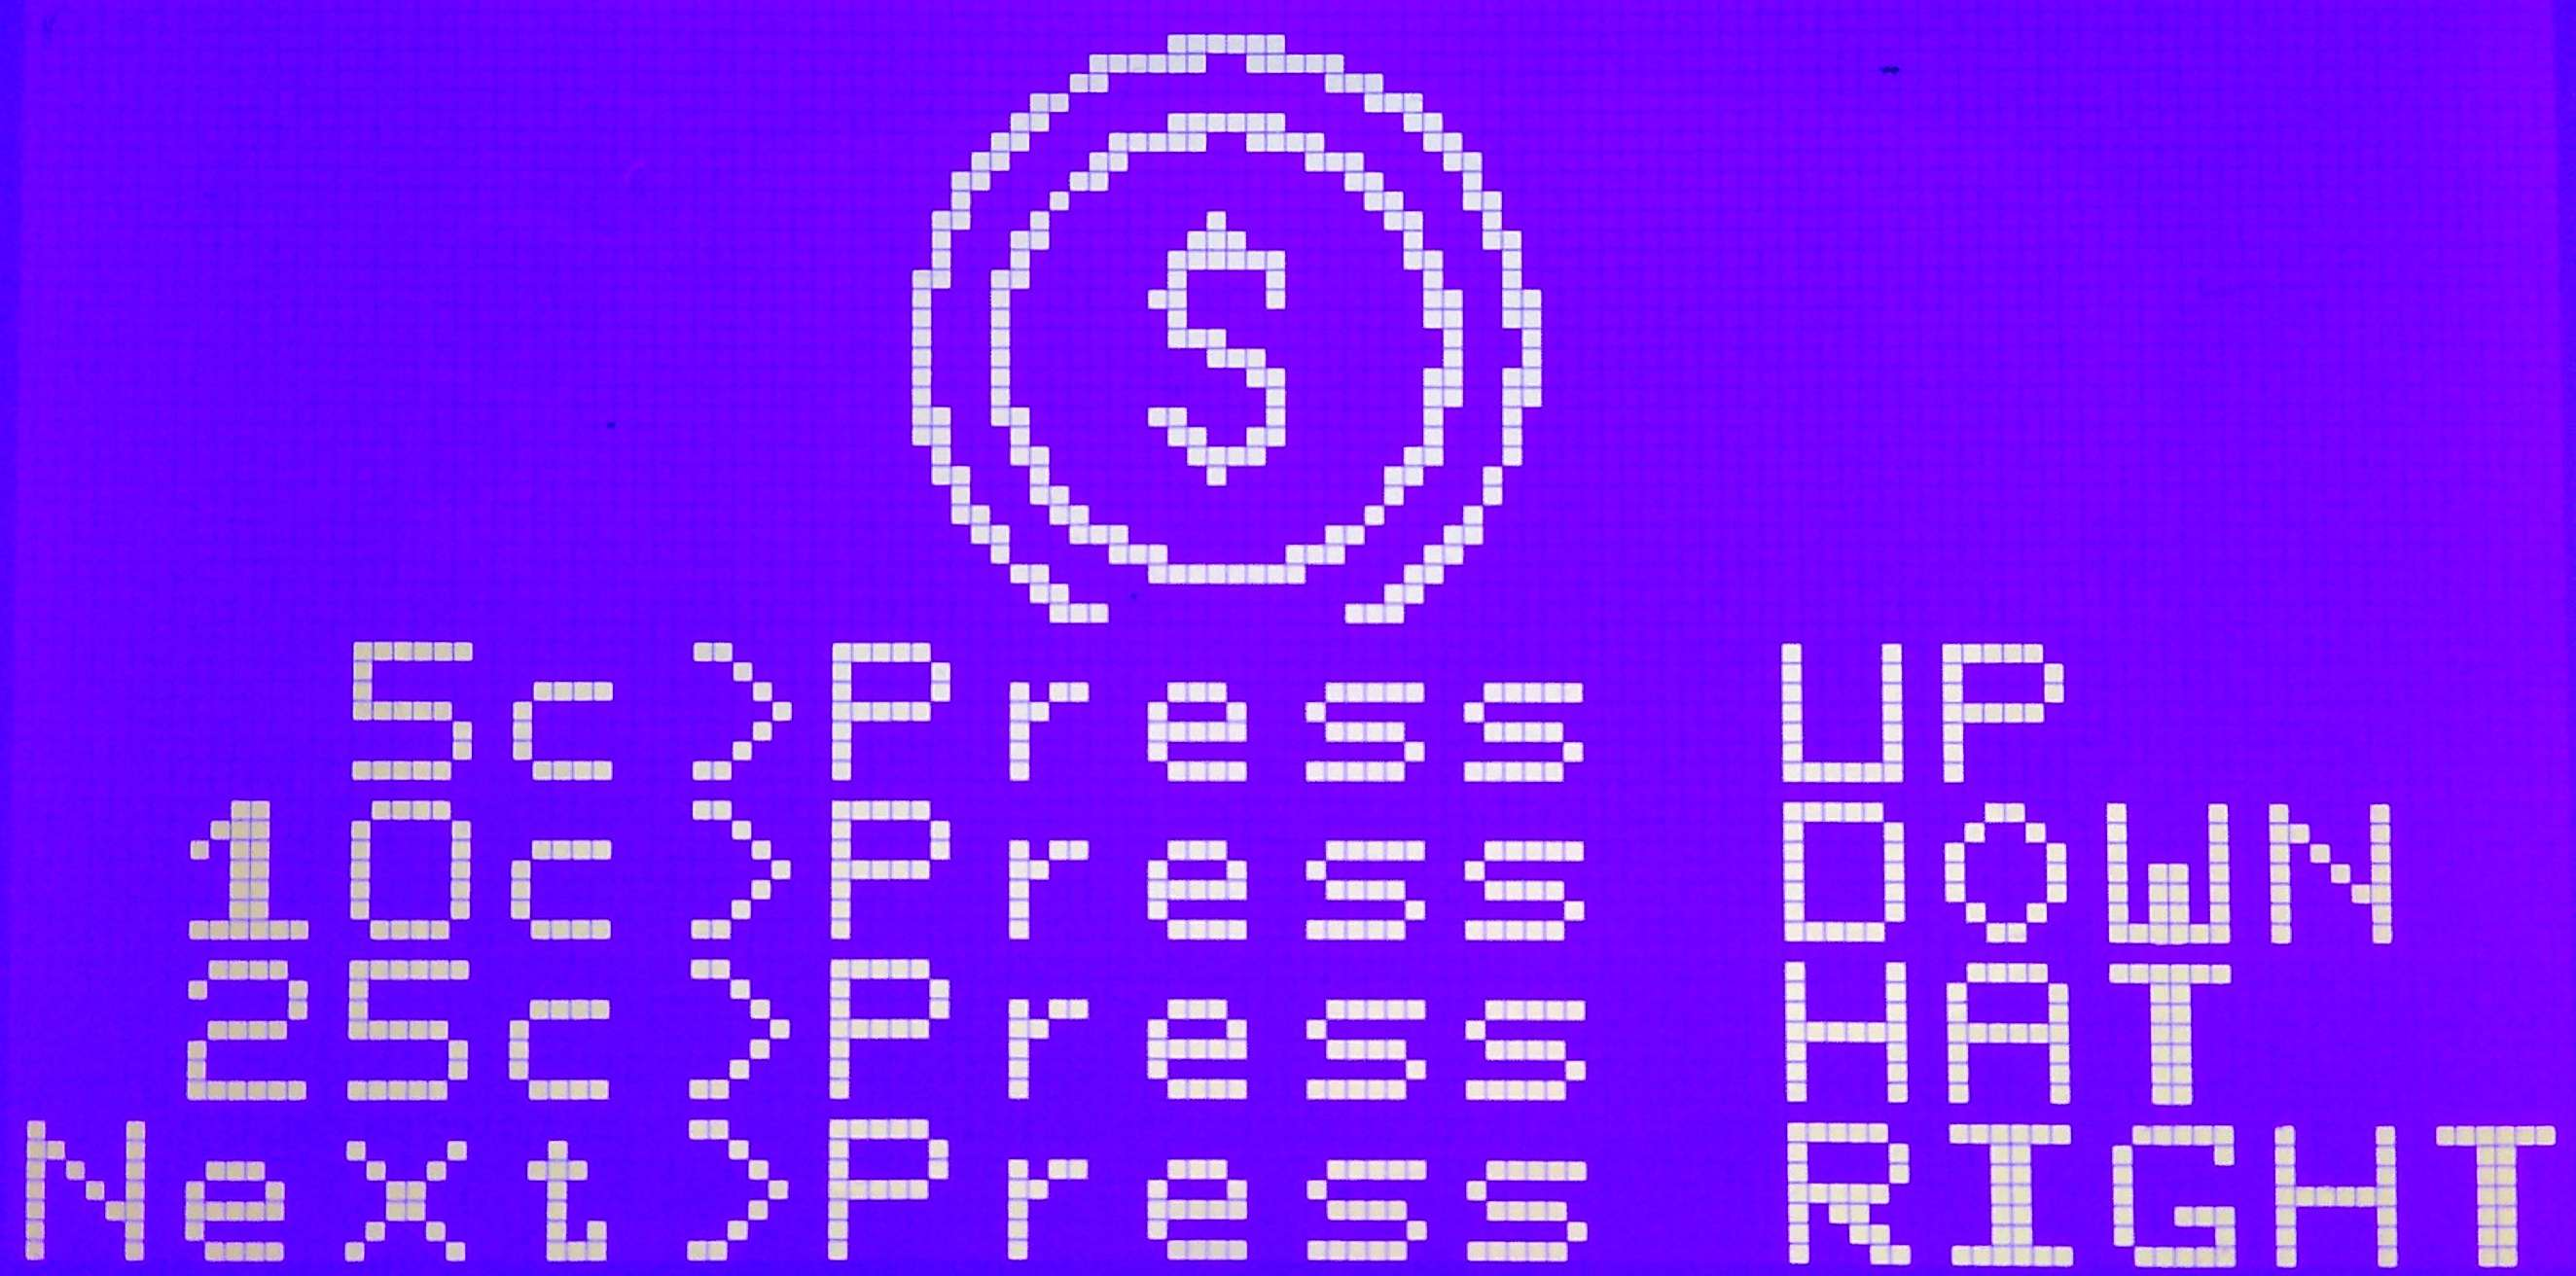
\includegraphics[width=8cm]{putcoin}
   \\Fig 1: Put Coin Screen(Initial)
   \\[2\baselineskip]
   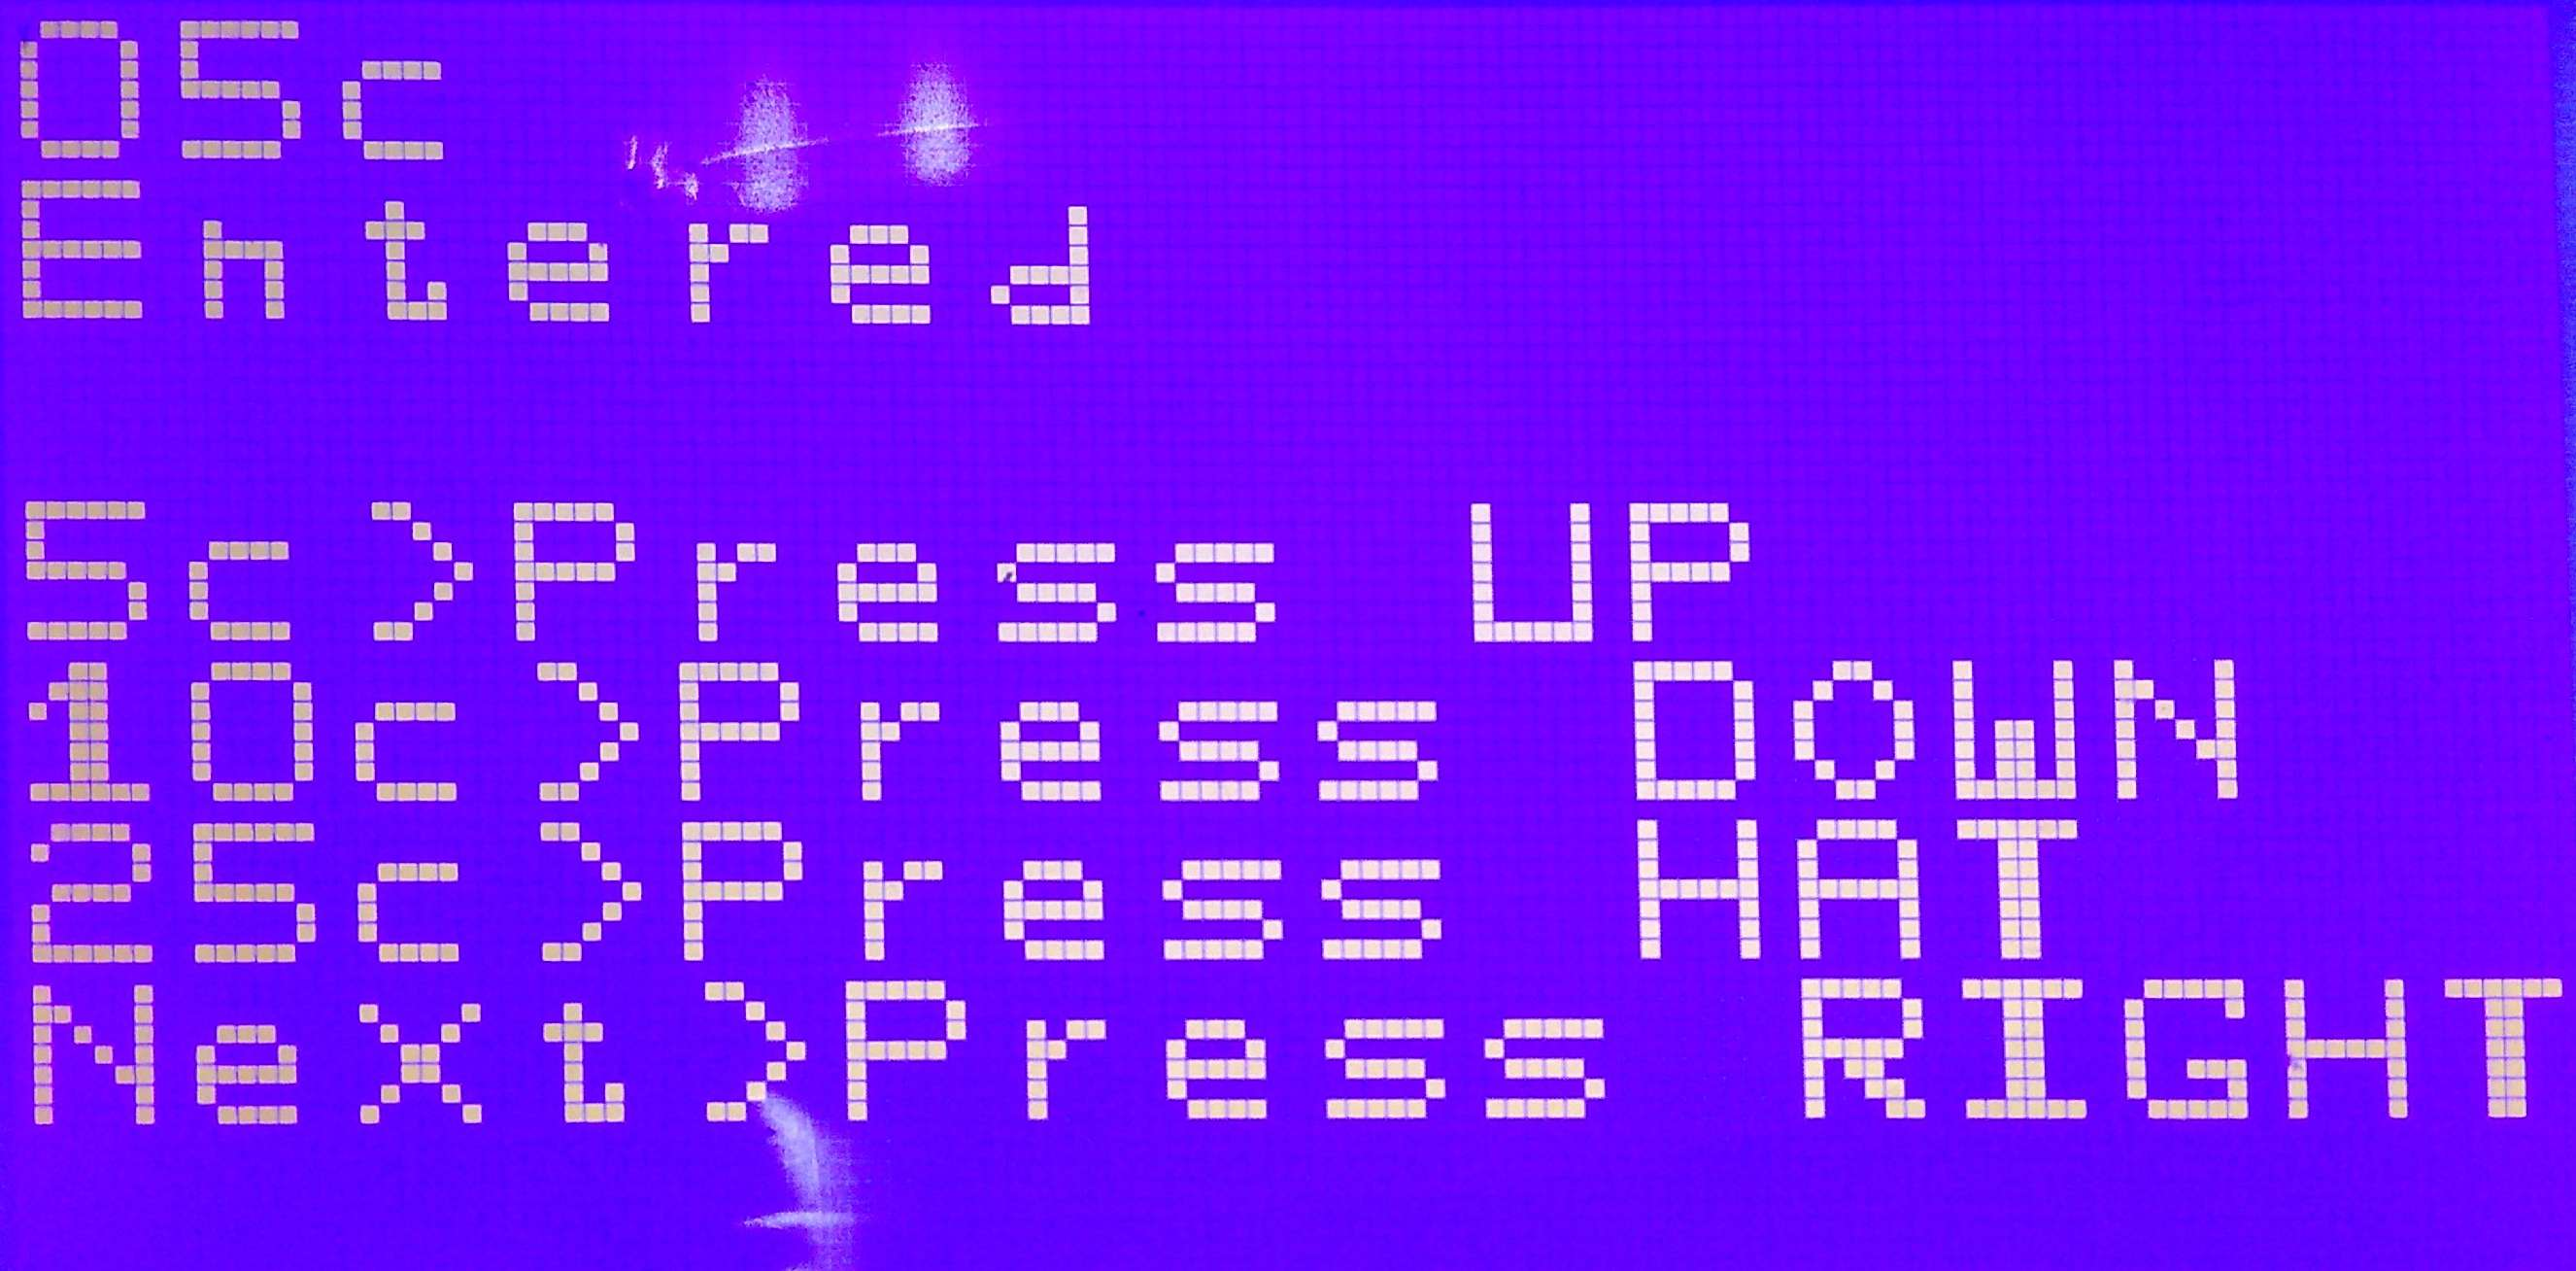
\includegraphics[width=8cm]{coinfive}
   \\Fig 2: Entered Dime Screen
   \\[2\baselineskip]
   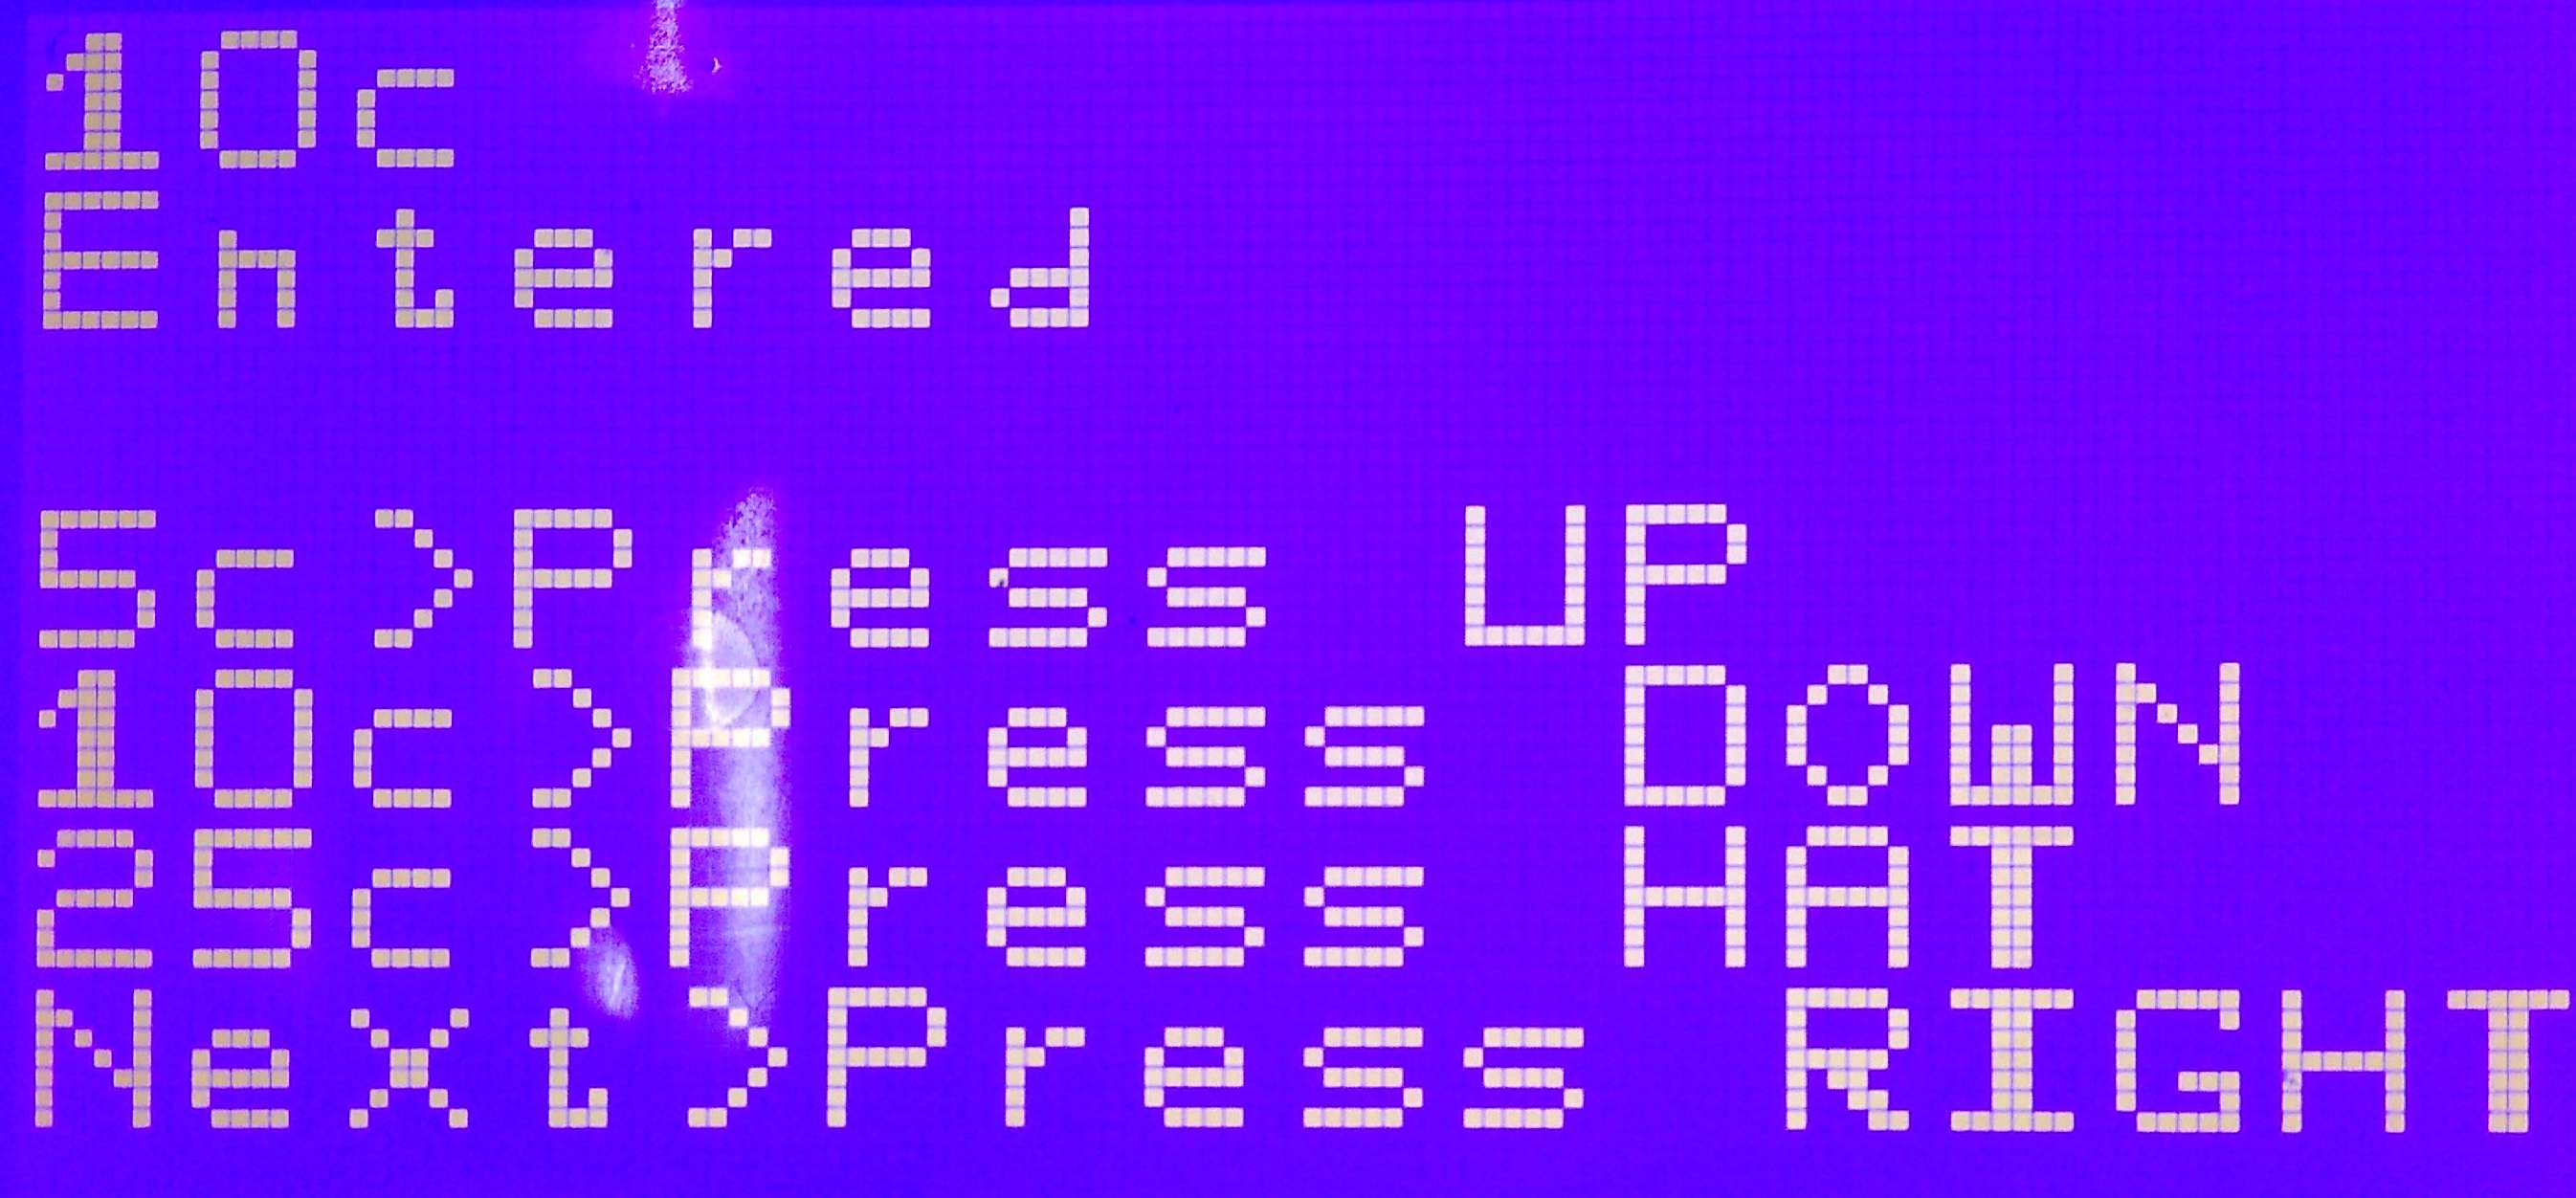
\includegraphics[width=8cm]{cointen}
   \\Fig 3: Entered Nickel Screen
   \\[2\baselineskip]
      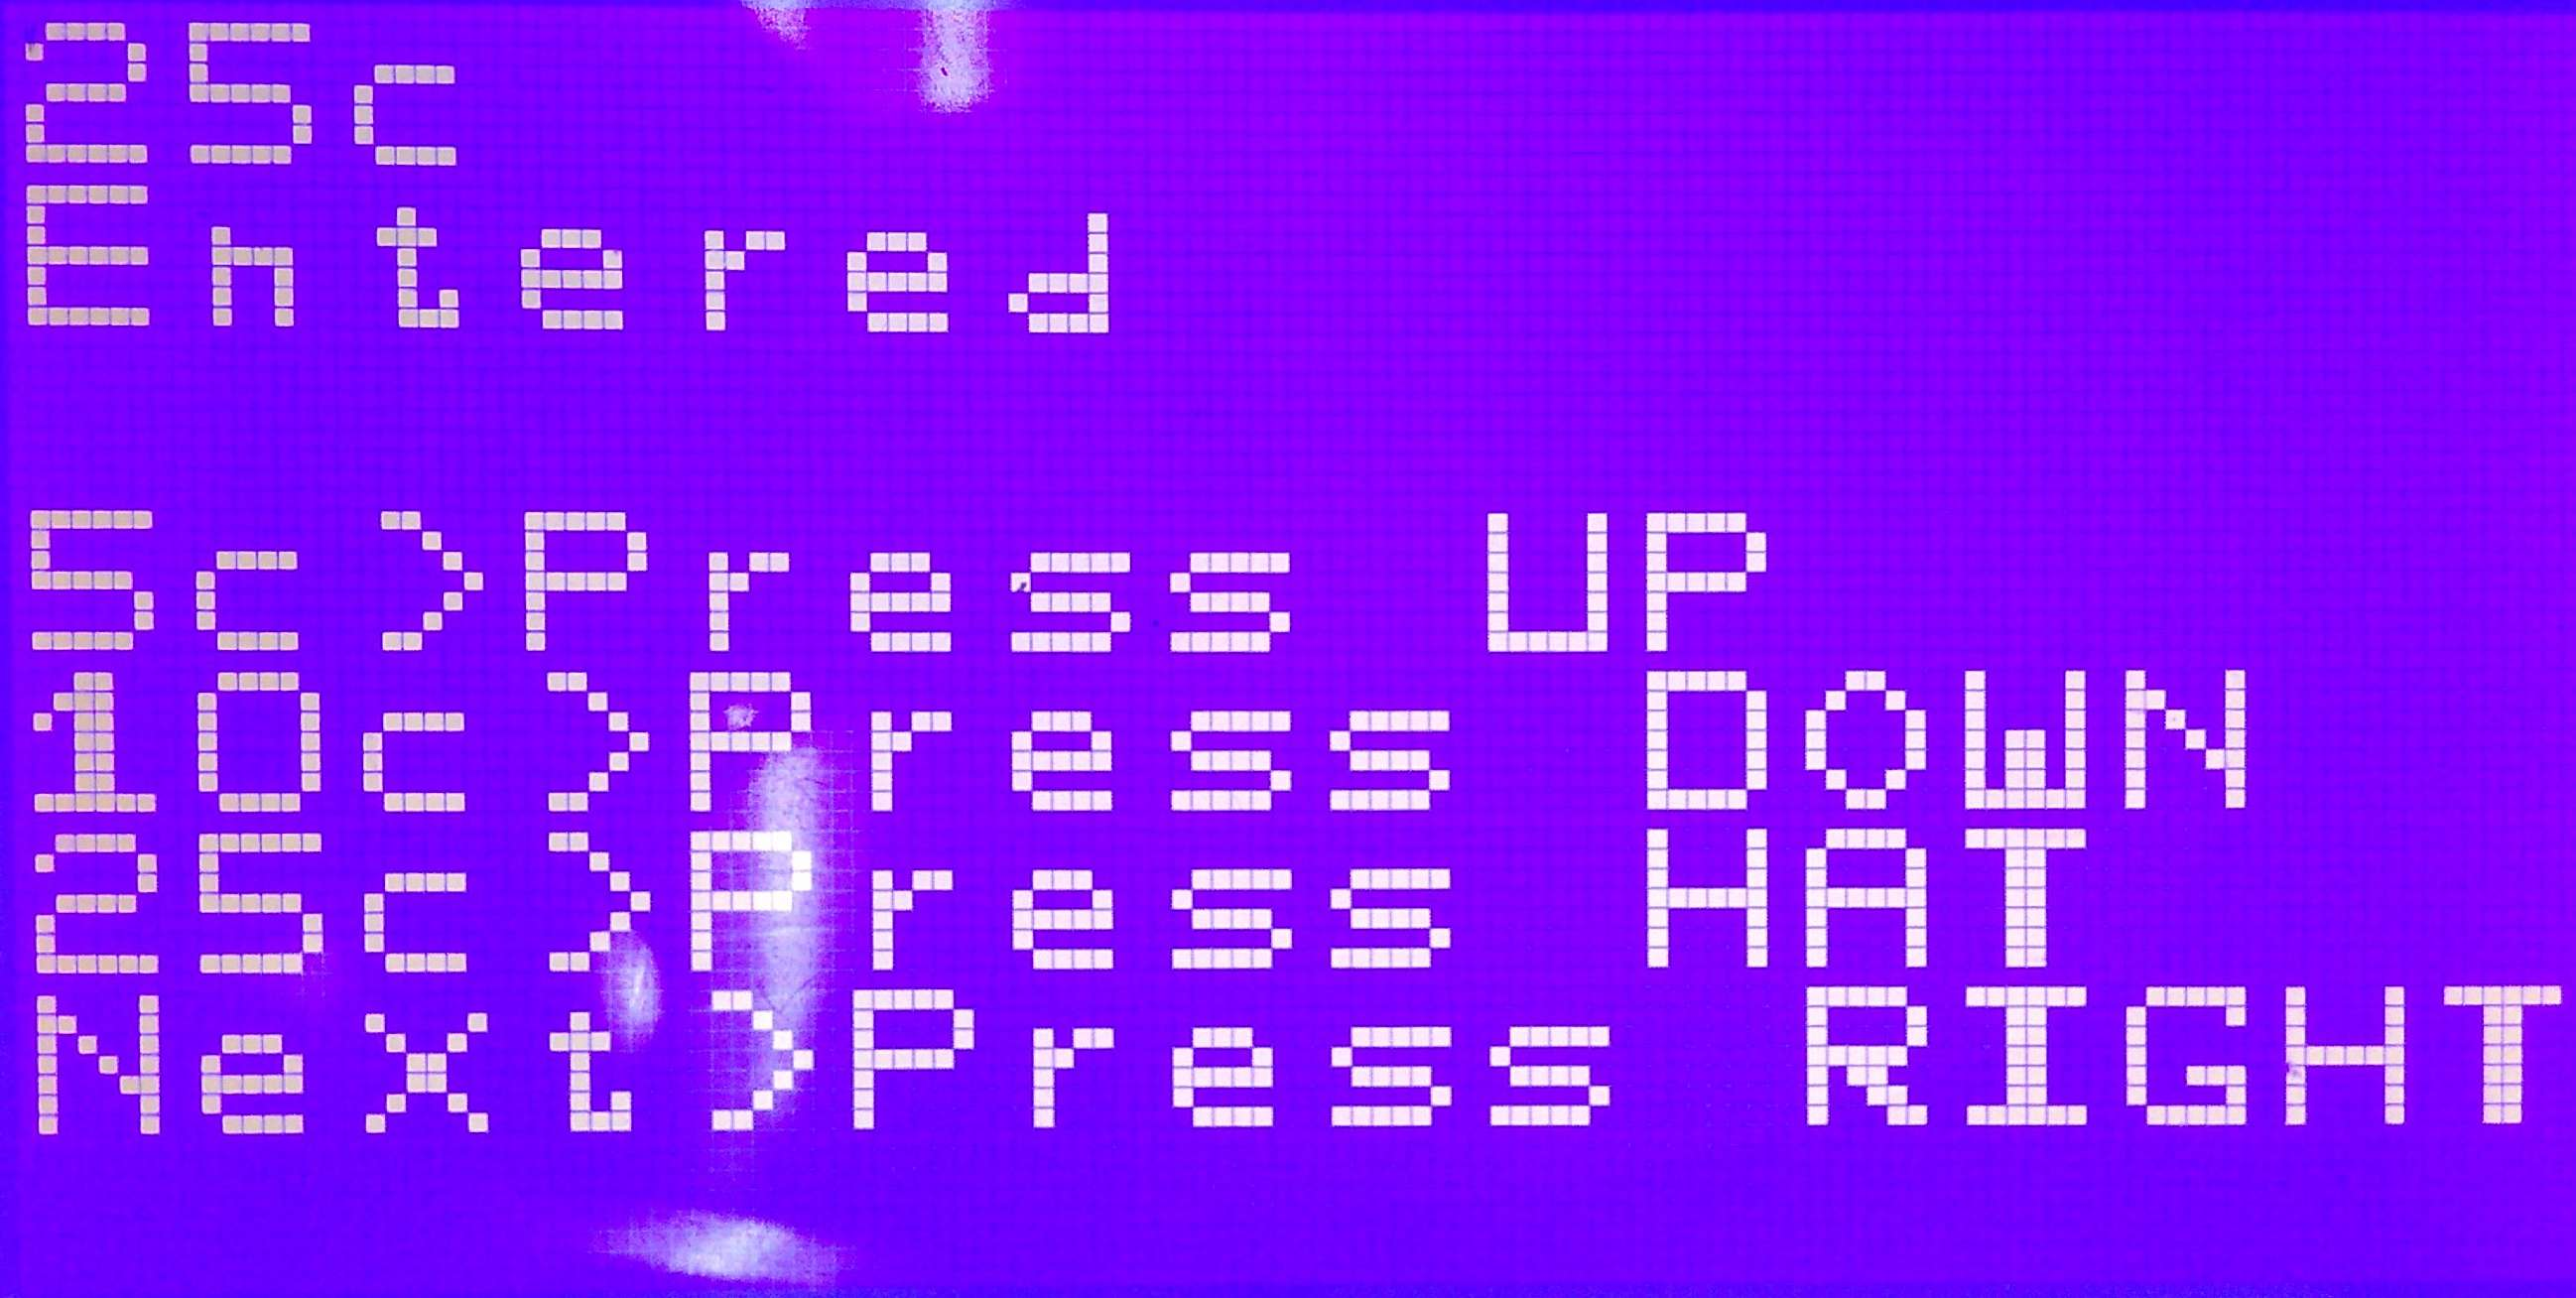
\includegraphics[width=8cm]{coinentered}
   \\Fig 4: Entered Quarter Screen
   \\[2\baselineskip]
 \end{center}
\subsubsection{SELECT:}
\begin{itemize}
    \item In \textit{SELECT} mode, initially, sode selection screen should be displayed with instructions to select each soda with appropriate switch press.  
    \item Once the requisite switch is pressed, the soda is selected.(And appropriate screen displayed as in Fig 6 and Fig 7). In case, multiple soda selection is allowed, increment each soda count variable.
    \item If the user changes his/her mind, he/she should be able to opt out. Hence, a cancel transaction option should be provided.(Fig 5 displays the cancel option)
    \item If cancel switch is pressed, ask for confirmation(as in Fig 8) and then move to \textit{CHANGE} substate in DELIVERY state. 
    \item Also, a transition switch should be provided to move on to \textit{DELIVERY} state.
\end{itemize}
\begin{center}
   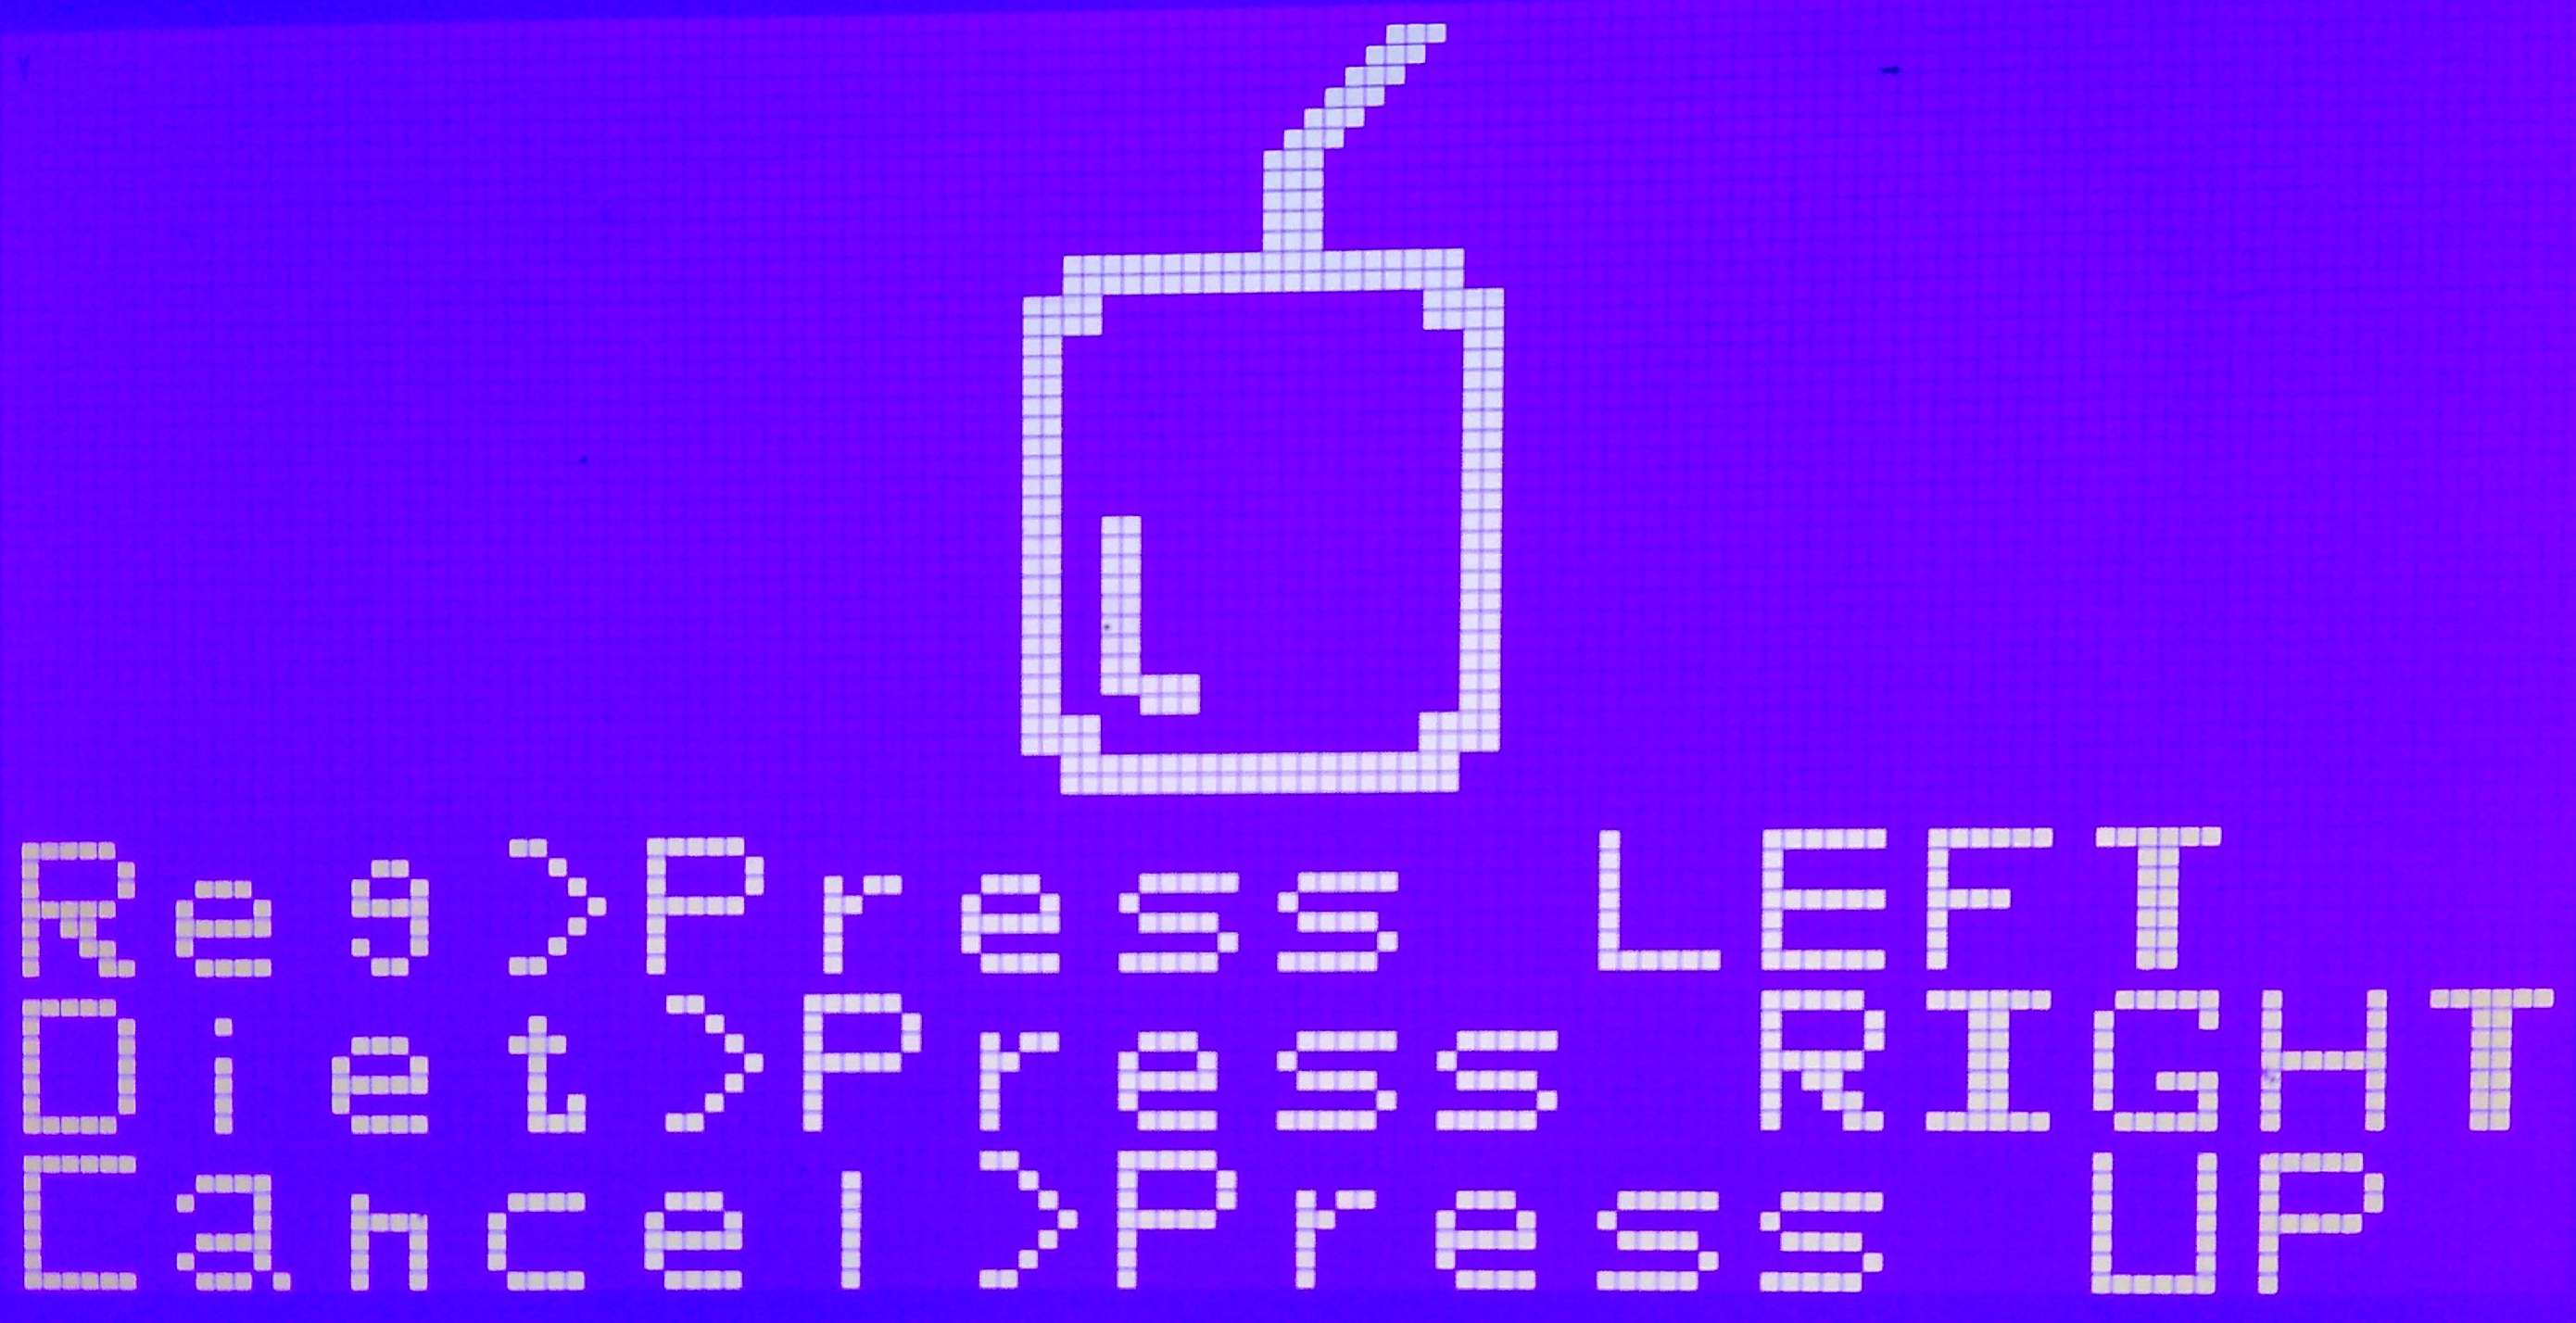
\includegraphics[width=8cm]{sodaselection}
   \\Fig5: Initial Soda Selection Screen
   \\[2\baselineskip]
   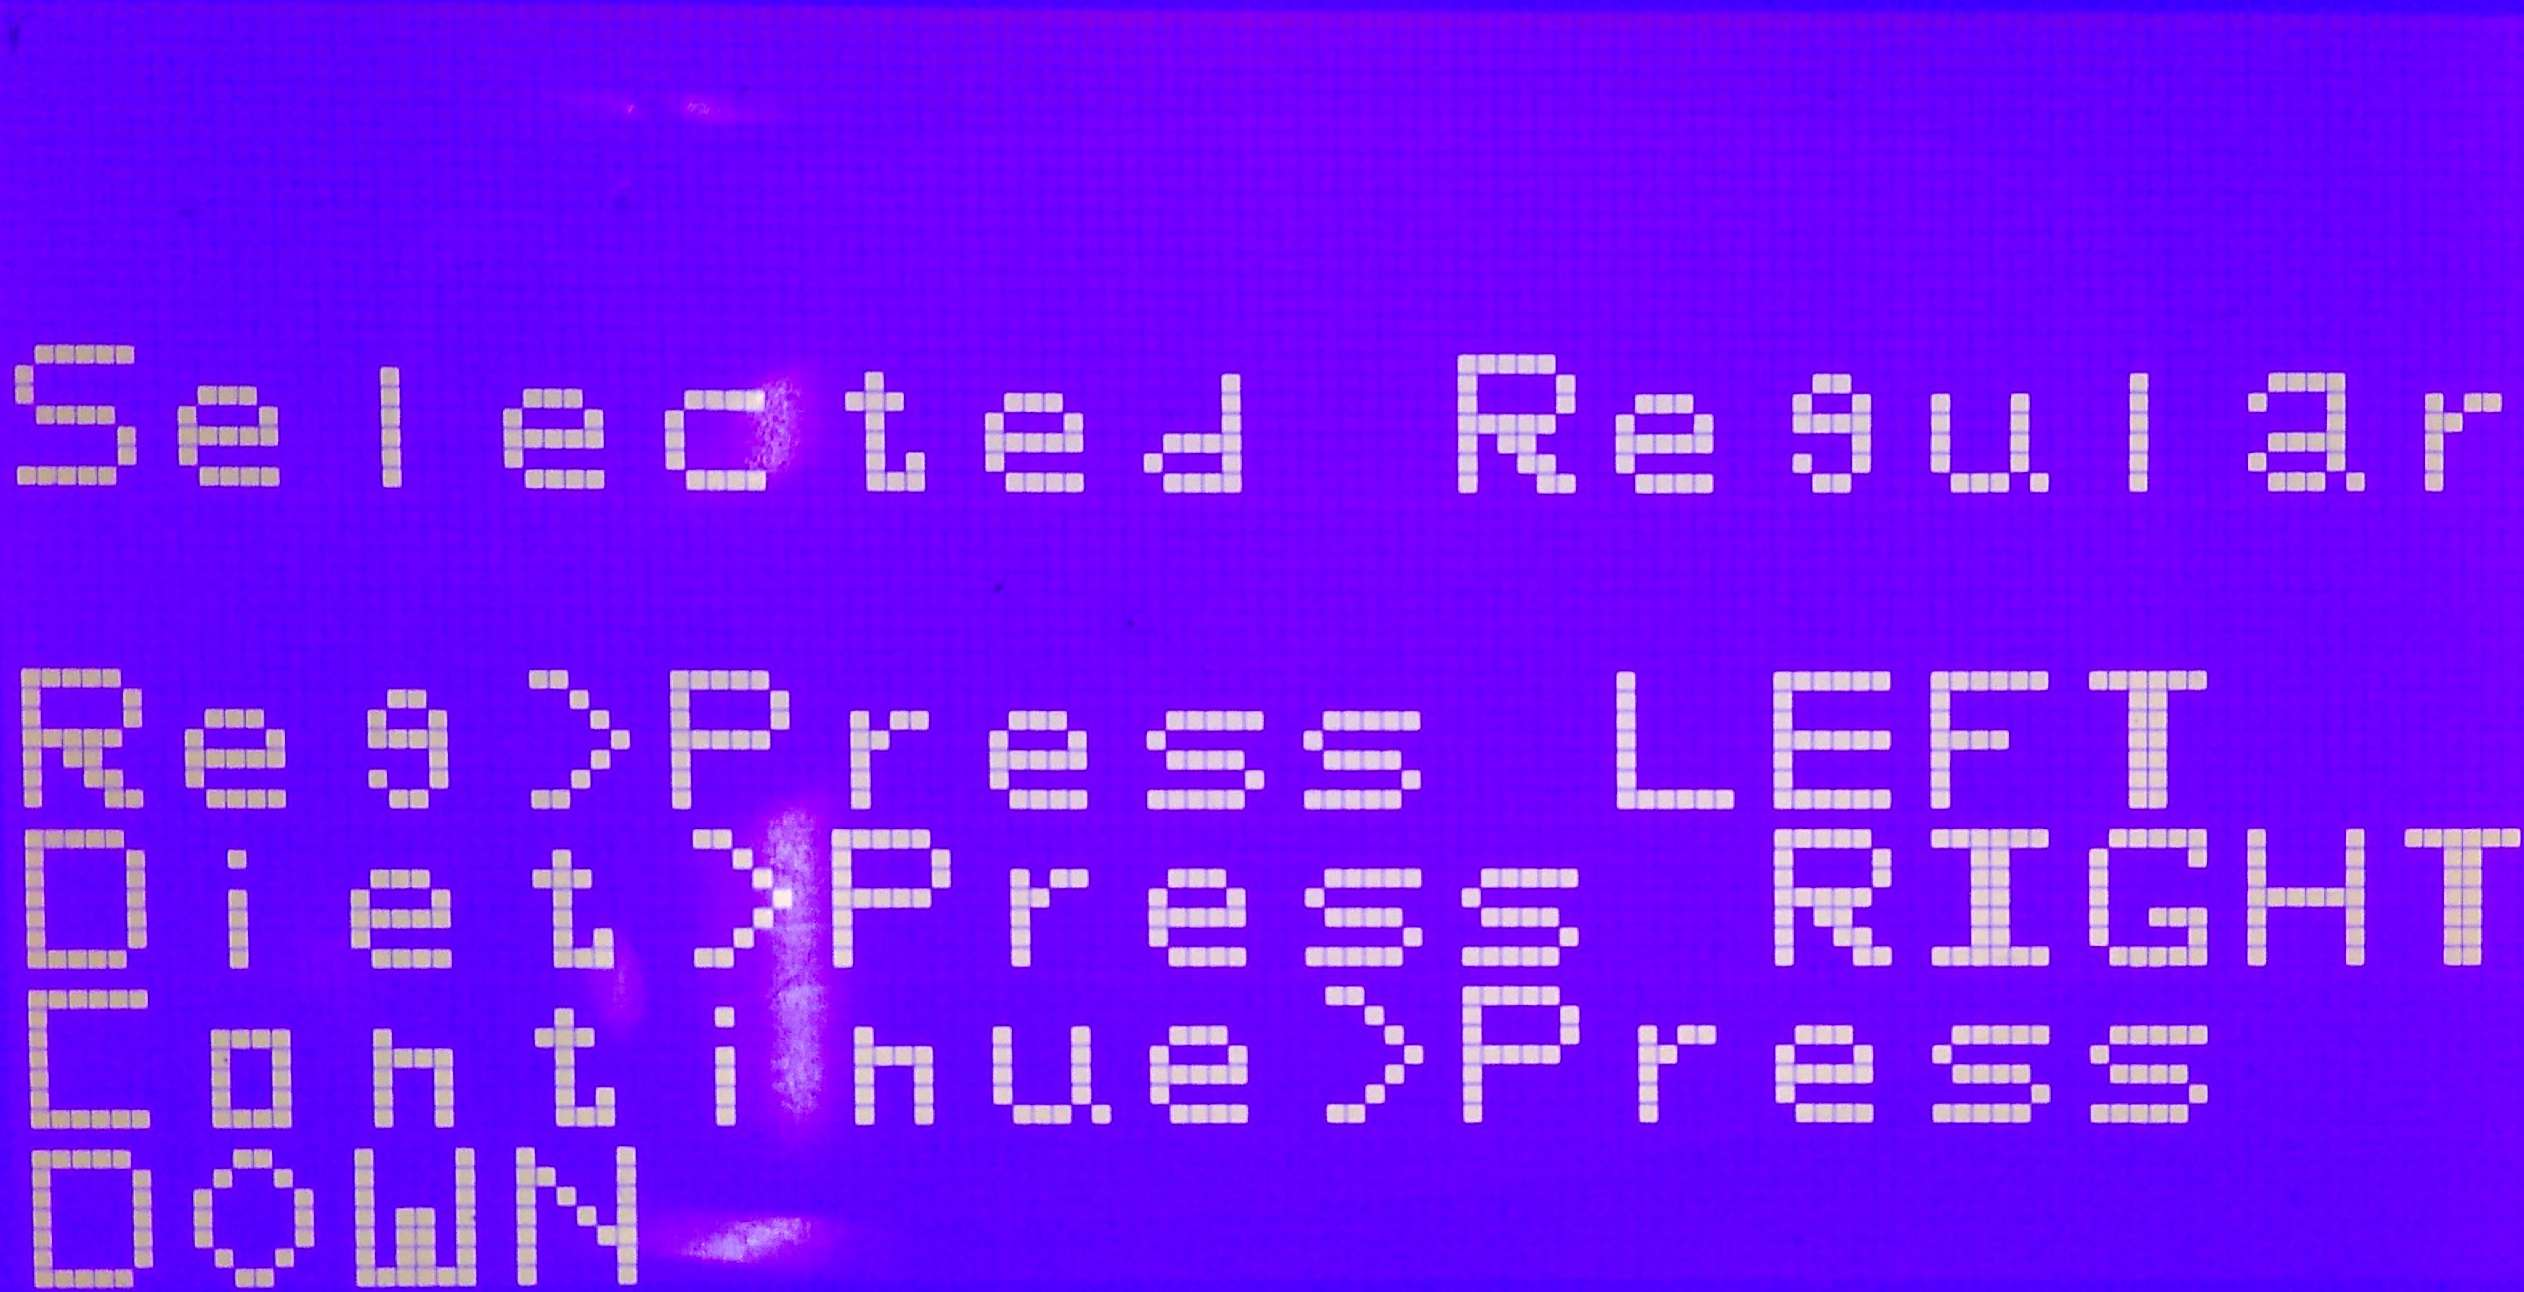
\includegraphics[width=8cm]{numbersoda}
   \\Fig6: Regular Soda Selected Screen
   \\[2\baselineskip]
   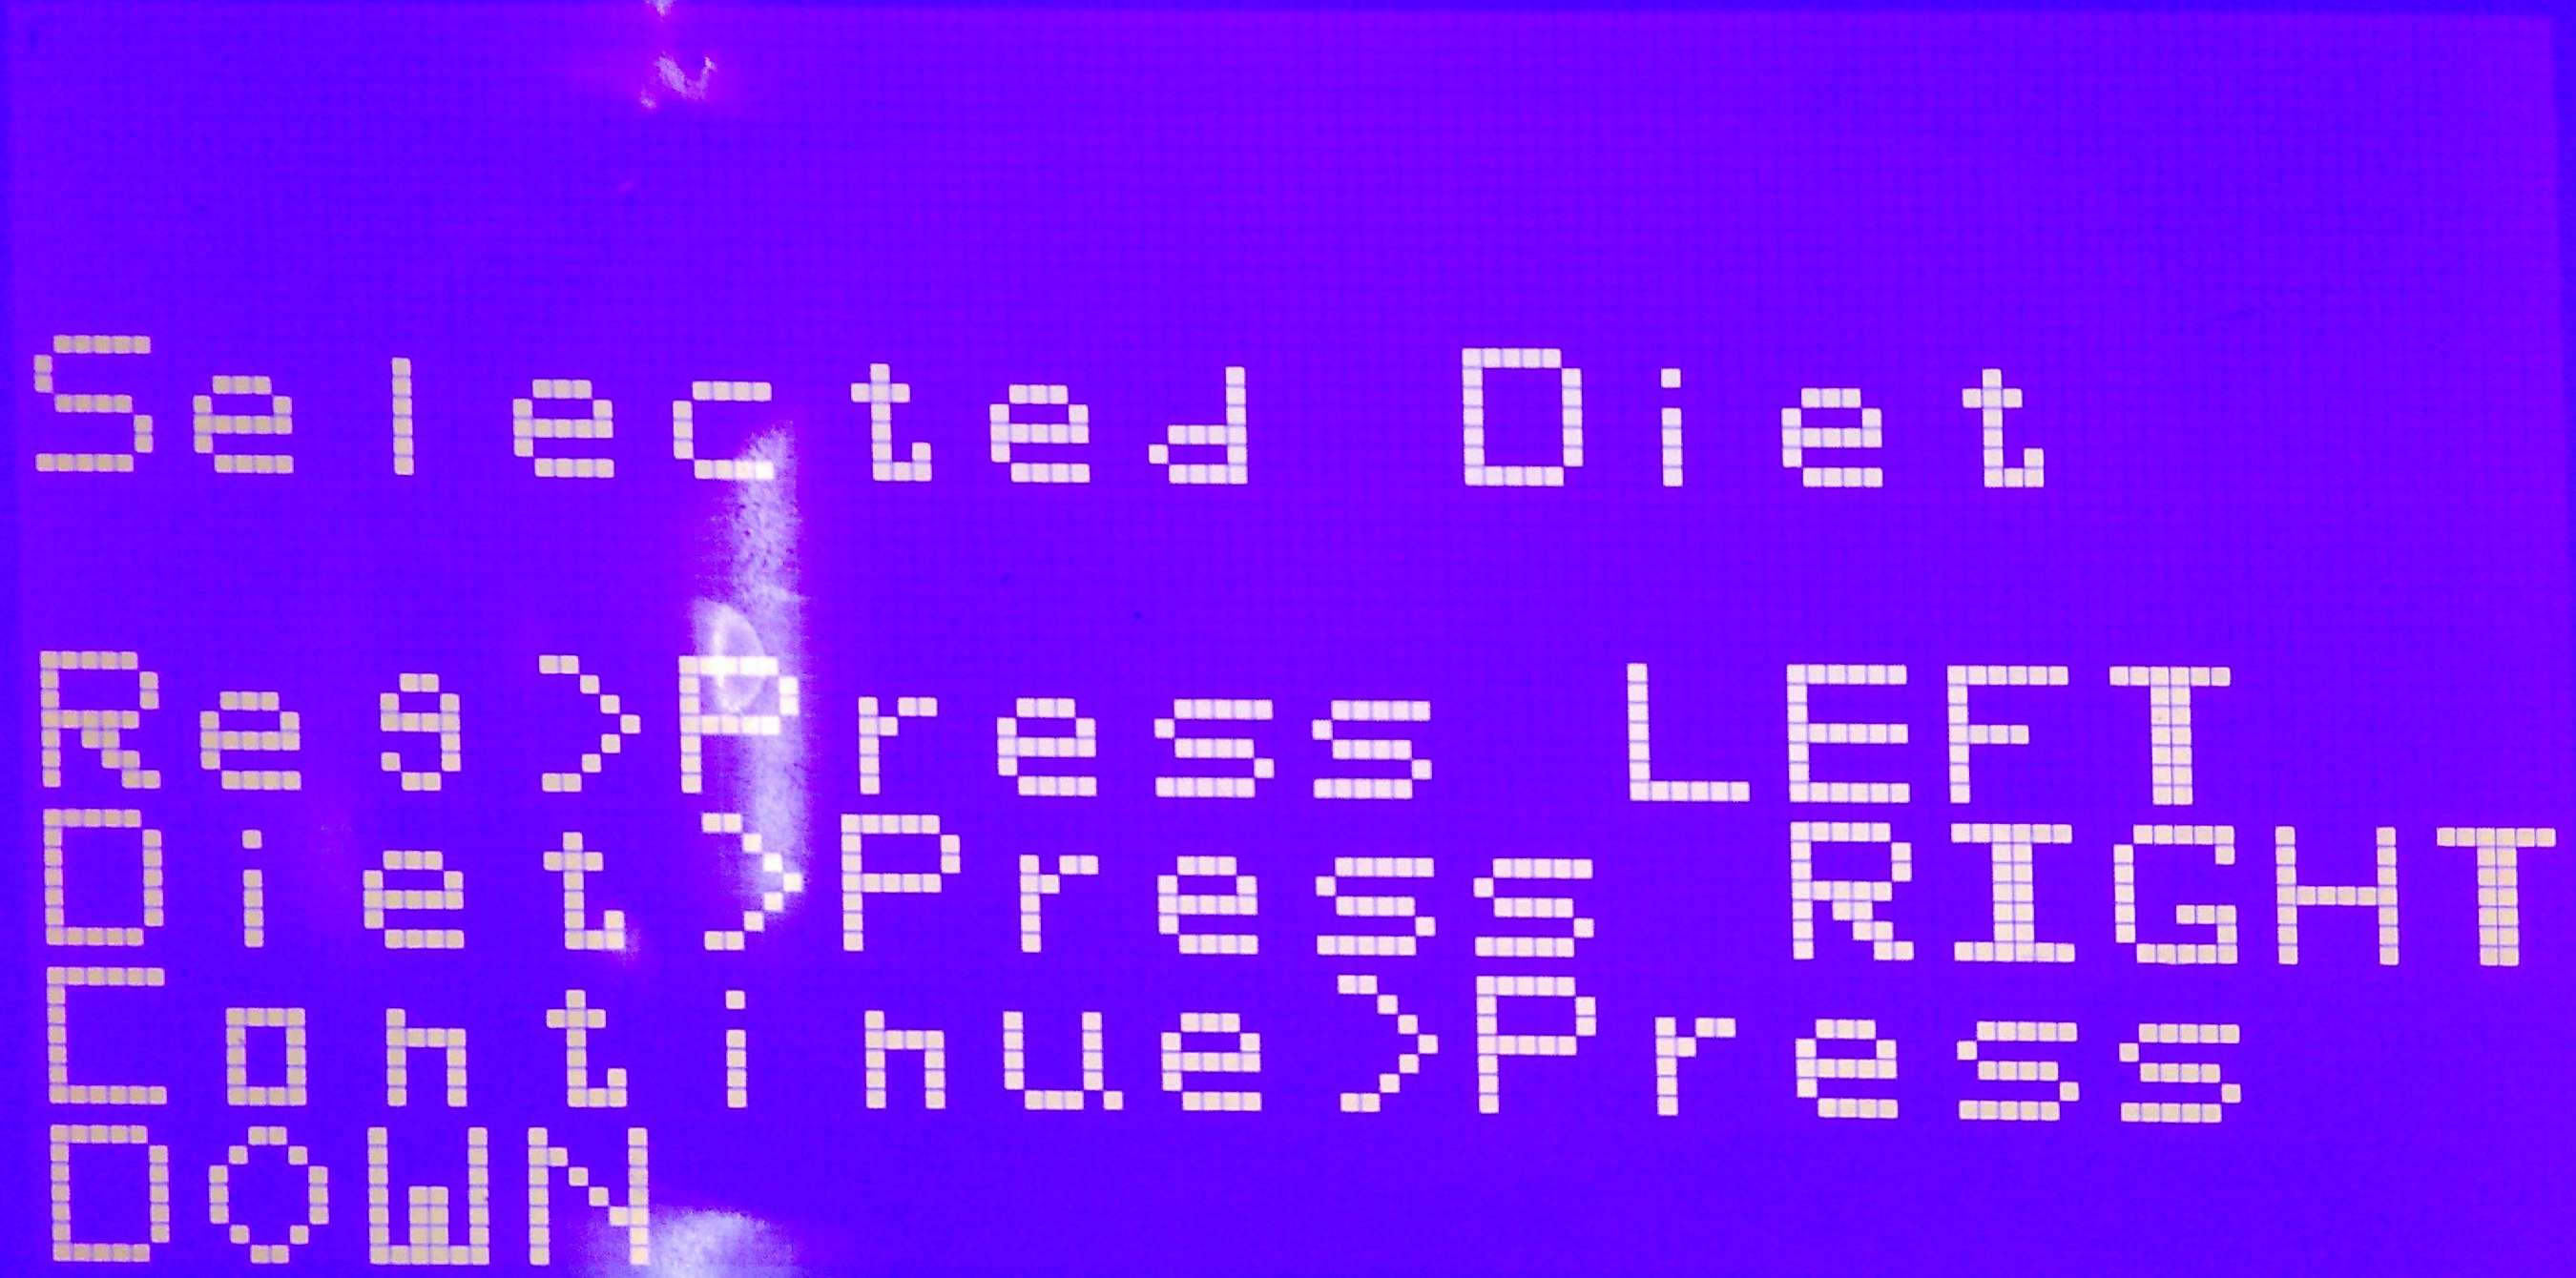
\includegraphics[width=8cm]{numbersoda2}
   \\Fig7: Diet Soda Selected Screen
   \\[2\baselineskip]
   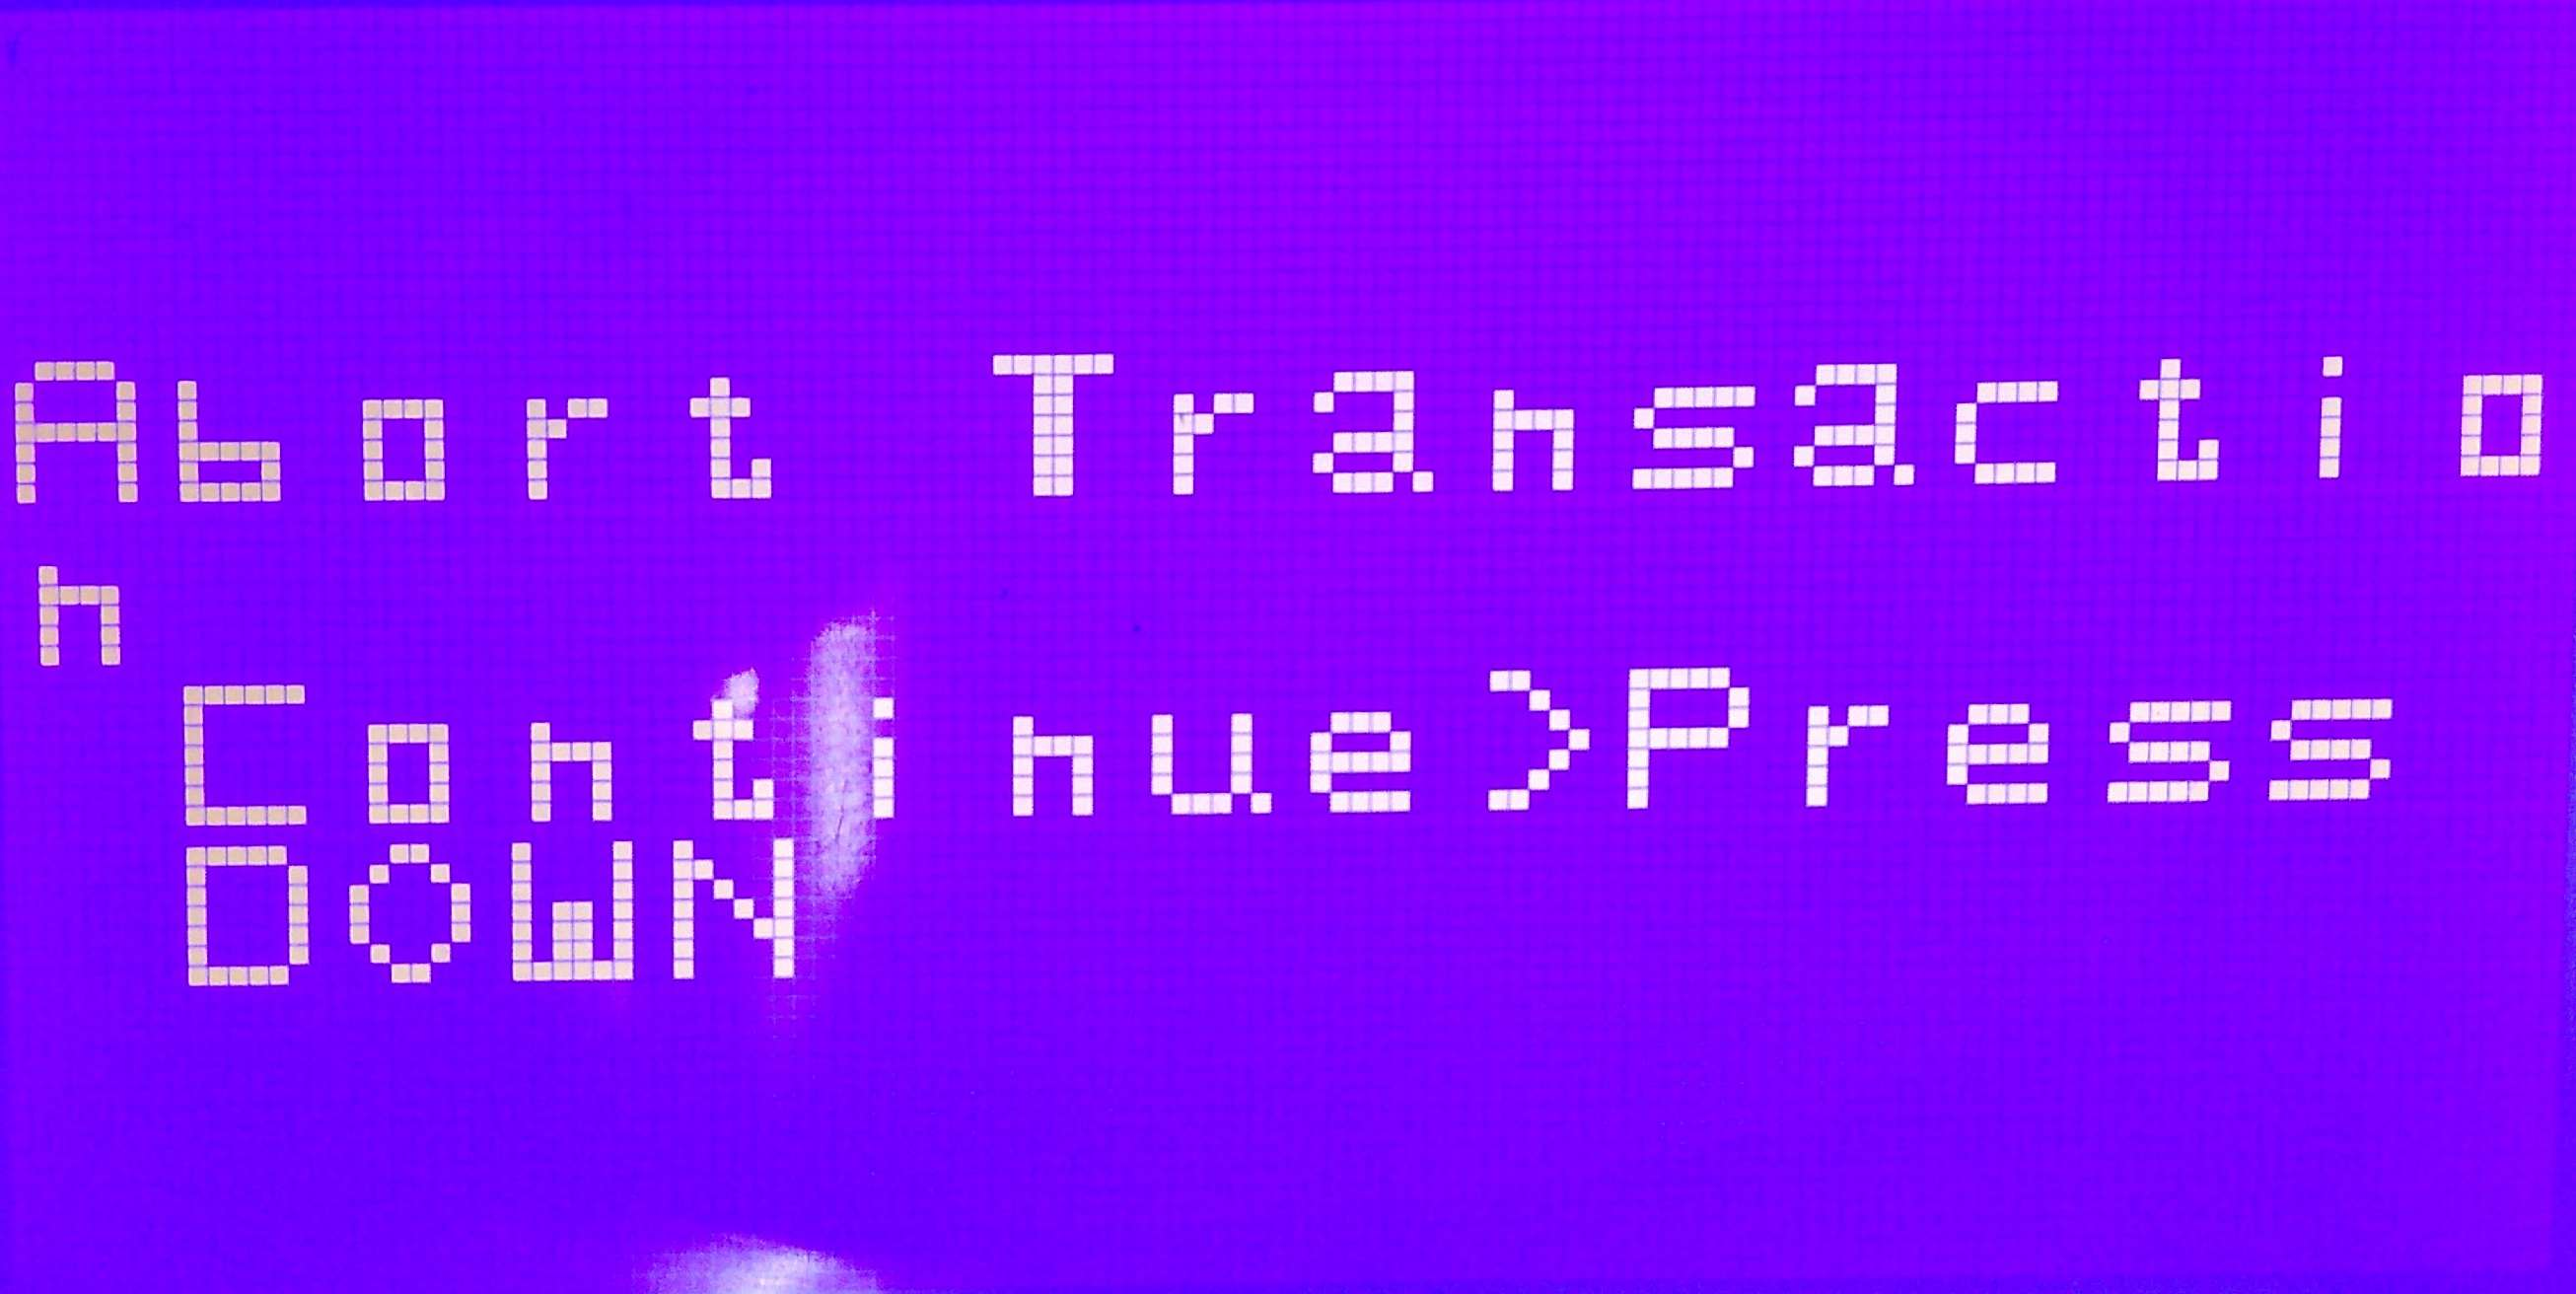
\includegraphics[width=8cm]{abort}
   \\Fig8: Abort Transaction Screen
   \\[2\baselineskip]
 \end{center}
\subsubsection{DELIVERY:}
\begin{itemize}
    \item Based on count of each soda selected, dispense corresponding soda through LED blink, and display the soda delivery screen(as in Fig 9).
    \item Once soda is delivered, return change such that each LED blink corresponds to 5¢. \textit{Number of LED Blinks = Sum/5}
    \item Notify the user of coin dispense using a screen(as in Fig 10)
\end{itemize}
\begin{center}
   
\includegraphics[width=8cm]{enjoydrink}
   \\Fig 9: Soda Dispense Screen
   \\[2\baselineskip]
   
\includegraphics[width=8cm]{collectchange}
   \\Fig 10: Change Dispense Screen
   \\[2\baselineskip]
    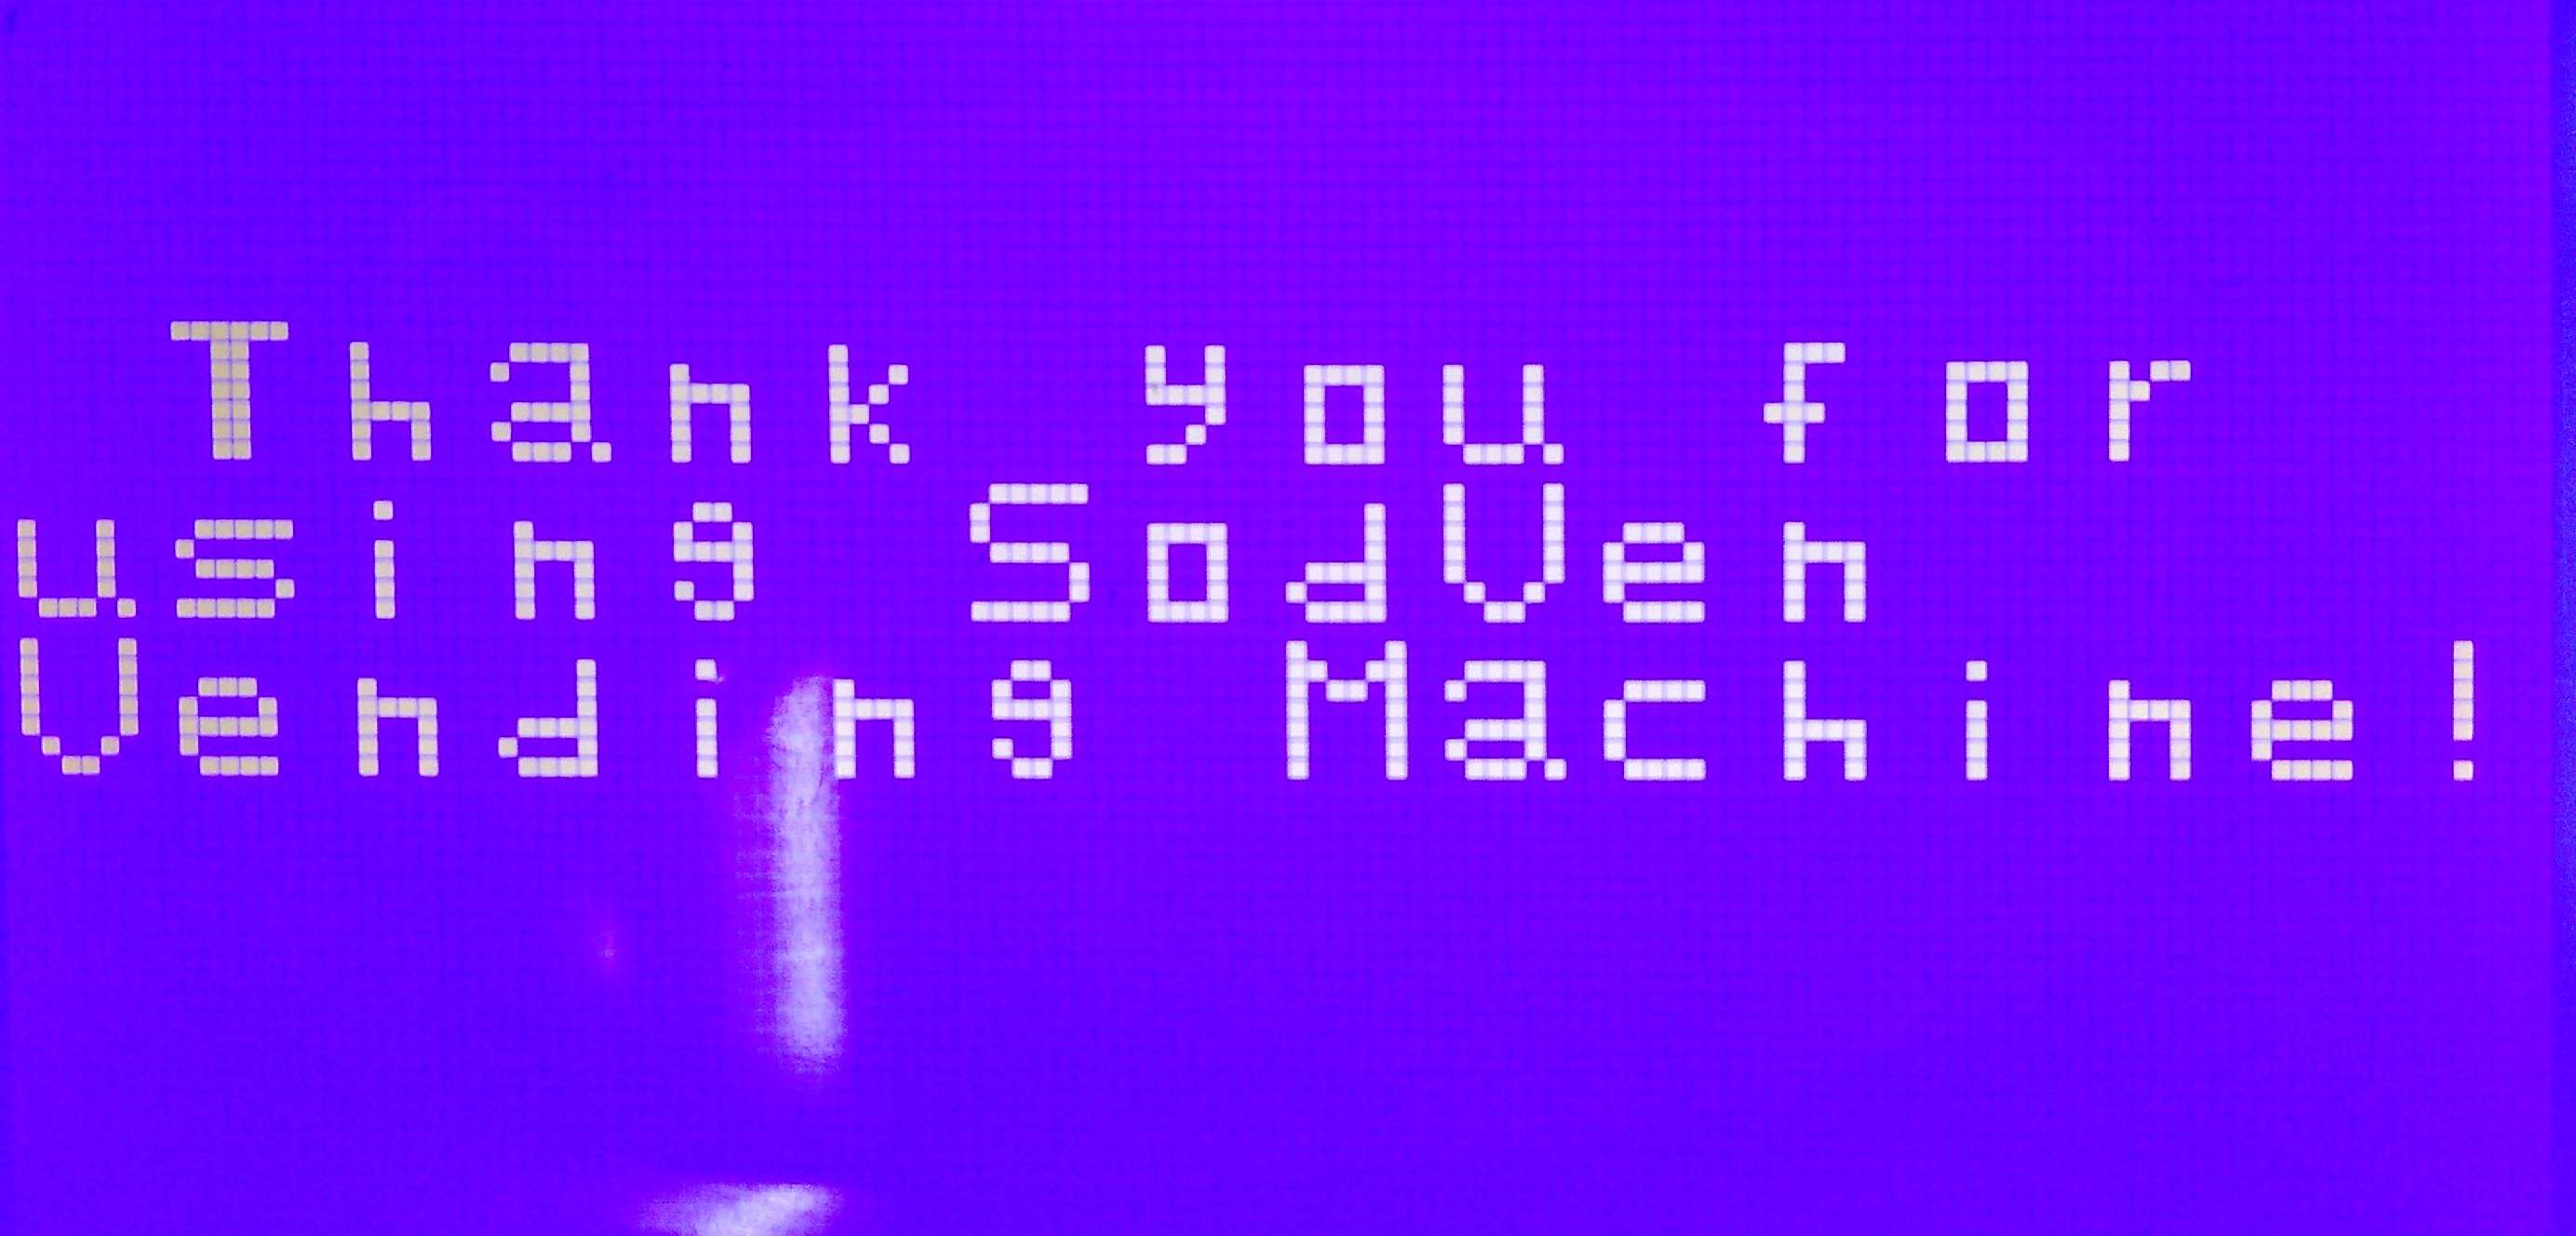
\includegraphics[width=8cm]{thanku}
   \\Fig 11: Thank You Screen
   \\[2\baselineskip]
 \end{center}
 \subsection{RTOS Implementation}
 \qquad Vending Machine can be implemented using two tasks \textit{readInput()} and \textit{displayOutput()}
 \subsubsection{readInput() Task}
 \qquad Handles all input switch press detection. Use Switch debouncing to accurately detect switch press. Since switch behaviour is different in different states, define switch behaviour accordingly in different states. Ex: UP Switch denotes Dime Enter in \textit{COIN} state(Fig 1), but cancels transaction in \textit{SELECT} state(Fig 5).
 \subsubsection{displayOutput() Task}
 \qquad Handles output screens to be displayed on GLCD corresponding to different states. Also handles LED output in \textit{DELIVERY} state. Ex: Coin Enter Screen in \textit{COIN} state(Fig 1), and Select Soda Screen in \textit{SELECT} state(Fig 5) are state-dependent.
\section{Procedure}
\begin{enumerate}
\item \qquad Include all the relevant header files in your code. Ensure that the following header
files are present:
\begin{lstlisting}[basicstyle = \small, language = C]
#include "Console/console.h"
#include "Console/glcd.h"
#include "Images/images.h"
\end{lstlisting}
\qquad The above libraries contain direct-to-GLCD font libraries and certain GUI graphic premade. The libraries can be downloaded from \href{https://github.com/eYSIP-2017/eYSIP-2017_Game_Development-TI-RTOS/blob/master/Documentation/VendingMachine/Console\%20Libraries.zip}{here}. Direct functions may be used to display for example, a coin, onto the screeen. Go through the headers to know more.
\item All necessary initialization, including Timers, Interrupts, Clock, GPIO, etc. can be performed using function \_init\_() from console.h. Edit console.h to initialize other peripherals in addition to the ones provided.
\item Initialize each of the various states using enumeration as in the following example:
\begin{lstlisting}[basicstyle = \small, language = C]
enum vm_modes{

    // States for Vending Machine

    INITM,
    COIN,
    SELECT,
    DELIVERY
};
// Initialization
enum vm_modes vm_mode = INITM;
\end{lstlisting}
\item Declare two tasks(empty), with corresponding semaphores \textit{readInput()} and \textit{displayOutput()}.
\item Use Timer 2A Interrupt for task scheduling and post semaphores at appropriate instances in time.
\item Now, in each task, implement the overall Vending Machine state machine, as in the statechart description given in Section 4(Switch Case or State Table Implementation can be used).
\end{enumerate}
\section{Demo and Submission:}
\begin{itemize}
    \item Implement appropriate statechart within each task and use appropriate task scheduling in RTOS.
    \item Show the output to TA and explain the working.
\end{itemize}
\begin{center}
\newline
   All The Best
  % \\[2\baselineskip]

 \end{center}
\end{document}
